\chapter{Architecture: Reinforcement Learning}
\label{chap:arch_rl}


% Chapter 17: replace the empty Architecture: Reinforcement Learning section.
% Requires existing textbook preamble with amsmath, amssymb, graphicx, tikz,
% and the existing calloutintuition / calloutpracticaltip environments.
% Figure drawings use only core TikZ (no special libraries).
\section{Architecture: Reinforcement Learning}\label{sec:rl}
Reinforcement learning (RL) learns a \textbf{policy} by interacting with an environment and improving decisions from their consequences.
Unlike supervised learning, the agent's actions change both subsequent observations and the data available for training; feedback may arrive many steps after the action responsible for it.
The central system is \emph{environment $\rightarrow$ experience $\rightarrow$ value estimate / advantage $\rightarrow$ policy update $\rightarrow$ environment}.
Section~4.7 already introduces the reward objective; this chapter explains how experience is generated, how an update becomes possible, and what researchers can change.

\begin{figure}[!htbp]\centering
\resizebox{.96\linewidth}{!}{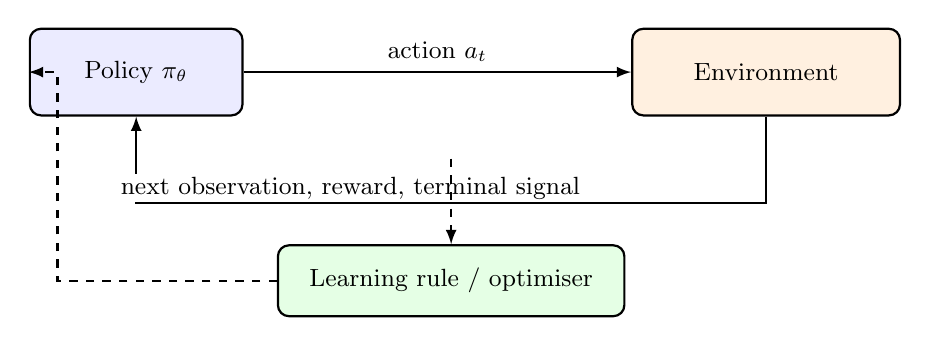
\begin{tikzpicture}[>=latex,thick,font=\small]
\node[draw,rounded corners,minimum width=27mm,minimum height=11mm,fill=blue!8] (agent) at (0,0) {Policy $\pi_{\theta}$};
\node[draw,rounded corners,minimum width=34mm,minimum height=11mm,fill=orange!12] (env) at (8,0) {Environment};
\draw[->] (agent) -- node[above]{action $a_t$} (env);
\draw[->] (env.south) -- ++(0,-1.1) -| node[pos=.33,above,fill=white,inner sep=1pt]{next observation, reward, terminal signal} (agent.south);
\node[draw,rounded corners,minimum width=44mm,minimum height=9mm,fill=green!10] (learn) at (4,-2.65) {Learning rule / optimiser};
\draw[->,dashed] (4,-1.1) -- (learn.north);
\draw[->,dashed] (learn.west) -- (-1.0,-2.65) -- (-1,0) -- (agent.west);
\end{tikzpicture}}
\caption{RL feedback loop. The policy acts; the environment changes; the resulting trajectory supplies training signals for a later update.}
\label{fig:rl-loop}
\end{figure}

\subsection{RL Foundations}\label{sec:rl-foundations}
An \textbf{agent} selects an action $a_t$ from an observation $o_t$ according to a policy $\pi_{\theta_{\mathrm{weights}}}(a_t\mid o_t)$.
The environment has a possibly hidden state $s_t$ and transition law $p(s_{t+1}\mid s_t,a_t)$; after the action it returns a reward $r_t$ and the next observation.
An \textbf{episode} is a trajectory $\tau=(o_0,a_0,r_0,o_1,a_1,r_1,\ldots)$ that ends at a task-defined terminal state or external cutoff.
A \textbf{Markov decision process} (MDP) assumes the current state contains the information needed to predict the next state given the action; a \textbf{partially observed MDP} (POMDP) supplies only $o_t$, making history or memory useful.
A contextual bandit is the special case in which actions affect immediate reward but not future decision states.

The policy maximises expected \textbf{return}, rather than fitting a labelled target action:
\[
\underbrace{J(\theta_{\mathrm{weights}})}_{\text{policy objective}}
=\mathbb E_{\tau\sim\pi_{\theta_{\mathrm{weights}}}}
\!\left[\underbrace{\sum_{t=0}^{N_{\mathrm{horizon}}-1}\gamma^t r_t}_{\text{discounted future reward}}\right],\qquad 0\leq\gamma\leq1.
\]
$\gamma$ controls how much distant reward matters; a smaller value shortens effective planning horizon but may prefer short-term gains.
An agent may receive a negative reward for one action yet correctly choose it because it enables a larger later return.
The feedback signal is an \emph{outcome}, not a correct action label; this creates delayed credit assignment and the need to explore.

\begin{figure}[!htbp]\centering
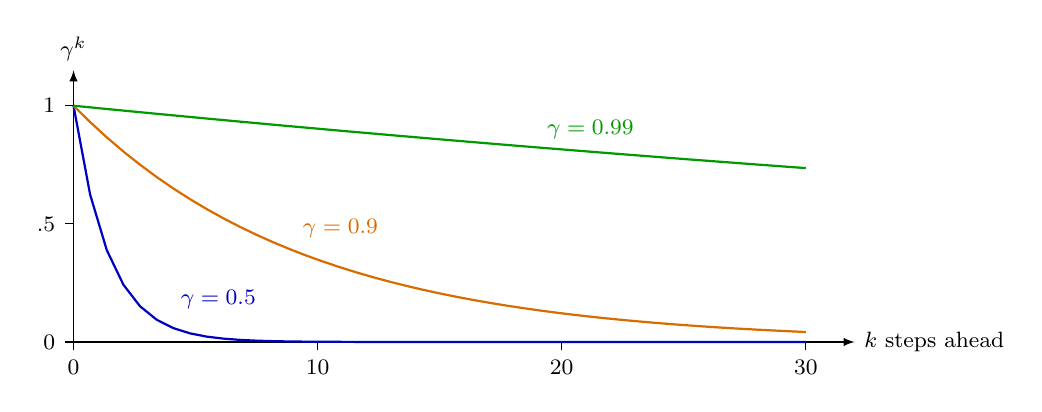
\begin{tikzpicture}[x=.31cm,y=3.0cm,>=latex,font=\footnotesize]
\draw[->] (0,0) -- (32,0) node[right]{$k$ steps ahead};
\draw[->] (0,0) -- (0,1.15) node[above]{$\gamma^k$};
\foreach \x in {0,10,20,30}{\draw (\x,0) -- (\x,-.035) node[below] {\x};}
\foreach \y in {0,.5,1}{\draw (0,\y) -- (-.35,\y) node[left] {\y};}
\draw[blue!75!black,thick] plot[domain=0:30,samples=45] (\x,{pow(.5,\x)});
\draw[orange!85!black,thick] plot[domain=0:30,samples=45] (\x,{pow(.9,\x)});
\draw[green!60!black,thick] plot[domain=0:30,samples=45] (\x,{pow(.99,\x)});
\node[blue!75!black,anchor=west] at (4,.18) {$\gamma=0.5$};
\node[orange!85!black,anchor=west] at (9,.48) {$\gamma=0.9$};
\node[green!60!black,anchor=west] at (19,.9) {$\gamma=0.99$};
\end{tikzpicture}
\caption{Discounting changes the effective planning horizon. A reward thirty steps later retains roughly $0.99^{30}\approx0.74$ of its weight at $\gamma=0.99$, versus $0.9^{30}\approx0.04$ at $\gamma=0.9$.}
\label{fig:rl-discount}
\end{figure}

\subsection{RL Environments}\label{sec:rl-environments}
An RL environment is an executable specification of \textbf{what the agent can observe, do, and be rewarded for}.
Environment design is a research decision: changing observations, dynamics or reward changes the task, often more than changing the policy network.
A simulator executes dynamics, an environment wraps these dynamics into an interaction task, a benchmark fixes evaluation conventions, and a training library updates the policy.
These components compose; they are not substitutes.

\paragraph{Developer contract.}
In Gymnasium-style environments \texttt{reset(seed=...)} returns an initial observation and information; \texttt{step(action)} returns \texttt{(observation, reward, terminated, truncated, info)}.
\texttt{terminated} means the modeled task ended; \texttt{truncated} means a time budget or external bound stopped the rollout.
This distinction affects a value target: an actual terminal state has no continuation value, whereas a timeout may still permit bootstrapping from the final state when continuing value is meaningful.
Code should also define observation/action spaces, valid actions, reset distributions, reproducible randomness, rendering, and diagnostic metadata.

\begin{figure}[!htbp]\centering
\resizebox{.98\linewidth}{!}{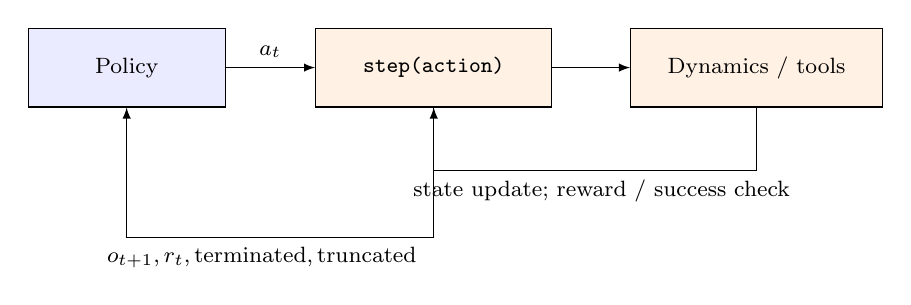
\begin{tikzpicture}[>=latex,font=\footnotesize]
\node[draw,fill=blue!8,minimum width=25mm,minimum height=10mm] (policy) at (0,0) {Policy};
\node[draw,fill=orange!10,minimum width=30mm,minimum height=10mm] (api) at (3.9,0) {\texttt{step(action)}};
\node[draw,fill=orange!10,minimum width=32mm,minimum height=10mm] (dyn) at (8,0) {Dynamics / tools};
\draw[->] (policy) -- node[above]{$a_t$} (api);
\draw[->] (api) -- (dyn);
\draw[->] (dyn.south) -- ++(0,-.8) -| node[pos=.24,below]{state update; reward / success check} (api.south);
\draw[->] (api.south) -- ++(0,-1.65) -| node[pos=.28,below]{$o_{t+1},r_t,\mathrm{terminated},\mathrm{truncated}$} (policy.south);

\end{tikzpicture}}
\caption{An environment is an interface plus dynamics and task semantics; the simulator is only one possible backend.}
\end{figure}

\paragraph{Environment design space.}
\begin{center}\begingroup\footnotesize\setlength{\tabcolsep}{3pt}
\begin{tabular}{|p{.19\linewidth}|p{.44\linewidth}|p{.28\linewidth}|}\hline
\textbf{Choice} & \textbf{Variables a developer changes} & \textbf{New limitation / failure}\\ \hline
Observation & True state vs sensors; noise; frame stacking; action history; privileged training inputs & Partial observability; leakage; larger input \\ \hline
Actions & Discrete/continuous; bounds; masking; control frequency; action chunks; tool calls & Invalid actions; long open-loop errors \\ \hline
Reward & Sparse/dense; shaping; penalties; verification; multi-objective weights & Proxy gaming; wrong optimum \\ \hline
Dynamics & Timestep; physical fidelity; stochasticity; random initial states; disturbances & Sim-to-real gap; slow rollouts \\ \hline
Episodes & Initial-state distribution; success/failure termination; time limit; curriculum & Shortcut learning; biased evaluation \\ \hline
\end{tabular}\endgroup\end{center}
\textbf{Inductive Bias.} If the observation exposes task-relevant state and the reward encodes actual success, the policy can learn useful behaviour; if either is a misleading proxy, greater optimisation may increase the wrong behaviour.
Reward shaping can accelerate sparse-reward learning but is not automatically policy-preserving; potential-based shaping is a special construction designed to preserve optimal policies under its assumptions.

\paragraph{Tools.}
\begin{center}\begingroup\footnotesize\setlength{\tabcolsep}{3pt}
\begin{tabular}{|p{.25\linewidth}|p{.34\linewidth}|p{.33\linewidth}|}\hline
\textbf{Layer / example} & \textbf{Used for} & \textbf{Research consideration}\\ \hline
Gymnasium / PettingZoo & Single-agent and multi-agent environment APIs (turn-based or parallel) & Consistent stepping, reset and agent scheduling\\ \hline
MuJoCo / MJX & Rigid-body contact dynamics and accelerated simulation & Fidelity, contact model, throughput, device support\\ \hline
Isaac Lab / ManiSkill & GPU-based robotics and manipulation training tasks & Robot/sensor complexity, many parallel environments, transfer\\ \hline
BrowserGym & Browser and software-agent tasks & Tool-side effects, task reset, measurable success\\ \hline
SB3 / CleanRL / TorchRL / RLlib & Training algorithms, collectors, replay and distributed rollouts & Baseline quality vs customisation and scaling\\ \hline
\end{tabular}\endgroup\end{center}
For robotic RL, the main systems choice is often how to combine sensor/physics fidelity with millions of sufficiently varied interaction steps.
For LLM tool agents, the ``environment'' can be a browser, test runner or sandbox: actions call tools, the state includes external software and reward may be a unit test or end-state verifier.
Multi-agent systems additionally choose simultaneous versus sequential moves, shared versus individual reward and whether other agents adapt during training.

\begin{figure}[!htbp]\centering
\resizebox{.98\linewidth}{!}{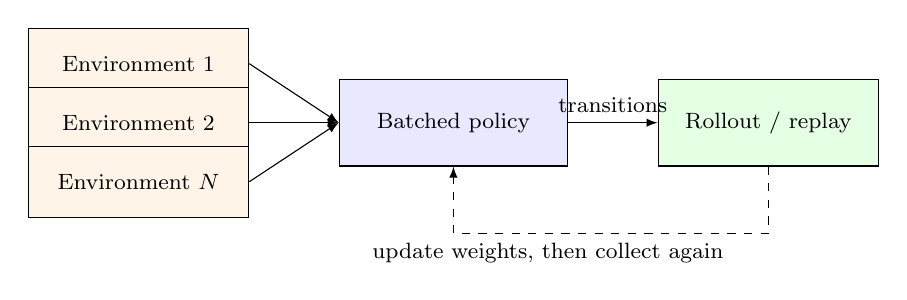
\begin{tikzpicture}[>=latex,font=\footnotesize]
\node[draw,fill=orange!9,minimum width=28mm,minimum height=9mm] (e1) at (0,0) {Environment 1};
\node[draw,fill=orange!9,minimum width=28mm,minimum height=9mm] (e2) at (0,-.75) {Environment 2};
\node[draw,fill=orange!9,minimum width=28mm,minimum height=9mm] (e3) at (0,-1.5) {Environment $N$};
\node[draw,fill=blue!9,minimum width=29mm,minimum height=11mm] (p) at (4,-.75) {Batched policy};
\node[draw,fill=green!10,minimum width=28mm,minimum height=11mm] (buf) at (8,-.75) {Rollout / replay};
\draw[->] (e1.east) -- (p.west); \draw[->] (e2.east) -- (p.west); \draw[->] (e3.east) -- (p.west);
\draw[->] (p) -- node[above]{transitions} (buf);
\draw[->,dashed] (buf.south) -- ++(0,-.85) -| node[pos=.35,below]{update weights, then collect again} (p.south);
\end{tikzpicture}}
\caption{Vectorised experience collection amortises inference and rollout overhead; asynchronous collectors increase throughput but may train with stale policies.}
\end{figure}
\begin{calloutpracticaltip}
Check environment semantics before debugging the optimiser: incorrect termination, reset leakage or reward implementation can make a broken experiment look successful.
\end{calloutpracticaltip}

\subsection{Credit Assignment and Value}\label{sec:rl-value}
A \textbf{value function} predicts the return obtainable from a state under a given policy, while an \textbf{action-value function} predicts it after taking a particular action:
\[
\underbrace{V^{\pi}(s_t)}_{\text{value of state}}
=\mathbb E_{\pi}\!\left[\sum_{k=0}^{\infty}\gamma^k r_{t+k}\mid s_t\right],\qquad
\underbrace{Q^{\pi}(s_t,a_t)}_{\text{value of action}}
=\mathbb E_{\pi}\!\left[r_t+\gamma V^{\pi}(s_{t+1})\mid s_t,a_t\right].
\]
The \textbf{Bellman relationship} says long-term value can be learned from an immediate reward and an estimate of the next state's value.
\textbf{Advantage}, $A^{\pi}(s,a)=Q^{\pi}(s,a)-V^{\pi}(s)$, measures whether an action did better than the state's usual baseline; it is useful because the policy should reinforce unusually good actions rather than all actions in high-reward states.

\begin{figure}[!htbp]\centering
\resizebox{.80\linewidth}{!}{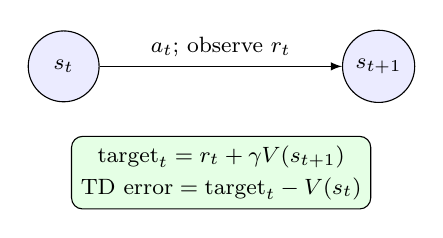
\begin{tikzpicture}[>=latex,font=\footnotesize]
\node[draw,circle,minimum size=9mm,fill=blue!8] (s) at (0,0) {$s_t$};
\node[draw,circle,minimum size=9mm,fill=blue!8] (sn) at (4,0) {$s_{t+1}$};
\draw[->] (s) -- node[above]{$a_t$; observe $r_t$} (sn);
\node[align=center,draw,fill=green!10,rounded corners] at (2,-1.35) {$\mathrm{target}_t=r_t+\gamma V(s_{t+1})$\\[2pt]$\mathrm{TD\ error}=\mathrm{target}_t-V(s_t)$};
\end{tikzpicture}}
\caption{Temporal-difference (TD) learning replaces a distant outcome with an immediate observation plus a bootstrapped continuation estimate.}
\end{figure}
\textbf{Monte Carlo} (MC) estimates return from a completed rollout: no bootstrap bias from a critic, but delayed, often high-variance feedback.
\textbf{TD learning} updates after each step using a value estimate: earlier and more frequent learning, but a wrong bootstrap target introduces bias and can propagate errors.
Exploration is a separate decision: $\epsilon$-greedy, entropy bonuses, optimistic estimates and intrinsic rewards encourage trying actions that might improve future knowledge.
\begin{calloutintuition}
Value predicts future return; advantage asks whether this action is better than the local default.
\end{calloutintuition}

\subsection{How RL Actually Learns}\label{sec:rl-learning}
\textbf{SARSA} learns $Q$ from the next action actually selected by the current policy, whereas \textbf{Q-learning} uses the best estimated next action irrespective of what the current exploratory policy would choose.
The resulting one-step targets are
\[
\underbrace{r_t+\gamma Q(s_{t+1},a_{t+1})}_{\text{SARSA: evaluate sampled next action}}
\quad\text{versus}\quad
\underbrace{r_t+\gamma\max_a Q(s_{t+1},a)}_{\text{Q-learning: greedy target}}.
\]
SARSA is on-policy in this standard formulation; Q-learning is off-policy.
With tabular values the update changes a stored entry; with \textbf{Deep Q-Networks (DQN)} a network predicts $Q_{\theta}(s,\cdot)$ and minimises squared TD error.
DQN adds a \textbf{replay buffer} to reuse and decorrelate stored transitions and a slowly updated \textbf{target network} to limit moving-target instability.
Experience replay improves sample efficiency but conflicts with strictly on-policy algorithms unless corrected or deliberately restricted to fresh batches.
The recurrent operational loop is \emph{collect trajectories $\rightarrow$ compute reward/value targets $\rightarrow$ update critic/policy $\rightarrow$ evaluate $\rightarrow$ repeat}.

\paragraph{An actual learning iteration.}
A rollout worker receives frozen policy weights, repeatedly queries the environment, and records $(o_t,a_t,r_t,o_{t+1},\mathrm{terminated},\mathrm{truncated},\log\pi_{\mathrm{old}}(a_t\mid o_t))$ when the algorithm requires those fields.
For DQN, sample transitions from replay, calculate a TD target with the target network, regress $Q_{\theta}$ towards it, and periodically refresh the target weights.
For PPO, collect a recent rollout, compute value targets and advantages, optimise several minibatch epochs against the stored action log-probabilities, then discard the batch before the next fresh collection.
For SAC, interleave new interactions with repeated replay-based critic and actor updates; the update-to-data ratio trades greater sample reuse against overfitting stale or narrow replay.
These are different \emph{data-flow systems}, even when all networks use AdamW from Section~8.7.

\subsection{Algorithm Evolution}\label{sec:rl-evolution}
RL is not one linear sequence like SGD to AdamW; different branches solve different credit-assignment, action-space and data-efficiency problems.

\begin{figure}[!htbp]\centering
\resizebox{.96\linewidth}{!}{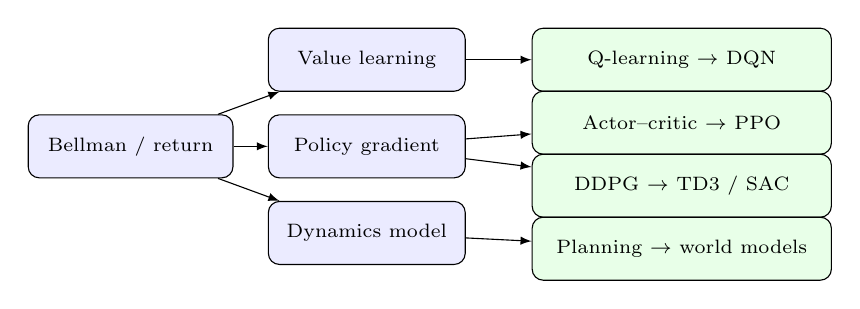
\begin{tikzpicture}[>=latex,font=\scriptsize]
\node[draw,rounded corners,fill=blue!8,minimum width=26mm,minimum height=8mm] (root) at (0,0) {Bellman / return};
\node[draw,rounded corners,fill=blue!8,minimum width=25mm,minimum height=8mm] (val) at (3,1.1) {Value learning};
\node[draw,rounded corners,fill=blue!8,minimum width=25mm,minimum height=8mm] (pol) at (3,0) {Policy gradient};
\node[draw,rounded corners,fill=blue!8,minimum width=25mm,minimum height=8mm] (mod) at (3,-1.1) {Dynamics model};
\node[draw,rounded corners,fill=green!9,minimum width=38mm,minimum height=8mm] (dqn) at (7,1.1) {Q-learning $\rightarrow$ DQN};
\node[draw,rounded corners,fill=green!9,minimum width=38mm,minimum height=8mm] (ppo) at (7,0.3) {Actor--critic $\rightarrow$ PPO};
\node[draw,rounded corners,fill=green!9,minimum width=38mm,minimum height=8mm] (sac) at (7,-.5) {DDPG $\rightarrow$ TD3 / SAC};
\node[draw,rounded corners,fill=green!9,minimum width=38mm,minimum height=8mm] (wm) at (7,-1.3) {Planning $\rightarrow$ world models};
\foreach \dst in {val,pol,mod}{\draw[->] (root) -- (\dst);}
\draw[->] (val) -- (dqn); \draw[->] (pol) -- (ppo); \draw[->] (pol) -- (sac); \draw[->] (mod) -- (wm);
\end{tikzpicture}}
\caption{The RL genealogy branches by what is learned and what data can be reused. Arrows show motivating ideas, not a claim that each method has only one predecessor.}
\end{figure}
\begin{center}\begingroup\footnotesize\setlength{\tabcolsep}{3pt}
\begin{tabular}{|p{.22\linewidth}|p{.35\linewidth}|p{.34\linewidth}|}\hline
\textbf{Step / branch} & \textbf{What changed and why} & \textbf{Benefit $\leftrightarrow$ cost}\\ \hline
Dynamic programming & Plan with known transitions/reward; Bellman backups & Exact model useful; typically unavailable or expensive\\ \hline
MC $\rightarrow$ TD & Bootstrap instead of waiting for full returns & Earlier updates; biased value targets\\ \hline
Q-learning $\rightarrow$ DQN & Replace table with network; replay and target network & Generalise over large observations; instability remains\\ \hline
REINFORCE $\rightarrow$ actor--critic & Direct policy gradient; learn a critic baseline & Handles continuous/stochastic actions; critic introduces bias\\ \hline
TRPO $\rightarrow$ PPO & Constrain policy movement; replace costly trust-region machinery with clipping & Repeated minibatch updates; clip is not a hard guarantee\\ \hline
DDPG $\rightarrow$ TD3 / SAC & Continuous off-policy actor--critic; twin critics/delayed updates or entropy-regularised stochastic actor & Sample reuse; greater tuning and value-estimation complexity\\ \hline
Dyna / MPC $\rightarrow$ world models & Predict outcomes to plan or simulate extra experience & Fewer real interactions; model bias compounds\\ \hline
\end{tabular}\endgroup\end{center}
\textbf{Policy-gradient} methods optimise sampled actions directly rather than evaluating all alternatives with $\max_aQ$, making continuous and structured action distributions natural.
The core score-function identity is
\[
\underbrace{\nabla_{\theta}J}_{\text{policy improvement direction}}
=\mathbb E_{\tau\sim\pi_{\theta}}\!\left[\sum_t\gamma^t
\underbrace{\nabla_{\theta}\log\pi_{\theta}(a_t\mid o_t)}_{\text{change sampled-action probability}}
\underbrace{A_t}_{\text{relative action value}}\right].
\]
The advantage should be treated as a learning signal (not differentiated through in a standard policy-gradient estimator).
A learned value baseline reduces gradient variance; biased advantages can change the update direction.
Generalised advantage estimation (GAE) combines TD errors across several horizons using a parameter $\lambda_{\mathrm{GAE}}$ to trade shorter, more biased estimates against longer, noisier ones.

\subsection{Deep RL Architectures}\label{sec:rl-architectures}
A \textbf{value-based} network maps observations to action values and then chooses an action; a \textbf{policy-based} network maps observations directly to action probabilities or continuous-action parameters.
\textbf{Actor--critic} splits the two roles: the actor generates actions while the critic assesses their expected return, often sharing an observation encoder.
The backbone can be an MLP for compact state vectors, a CNN for images, an RNN for partial observations, or a Transformer for long trajectories; the RL objective does not prescribe the architecture.

\begin{figure}[!htbp]\centering
\resizebox{.98\linewidth}{!}{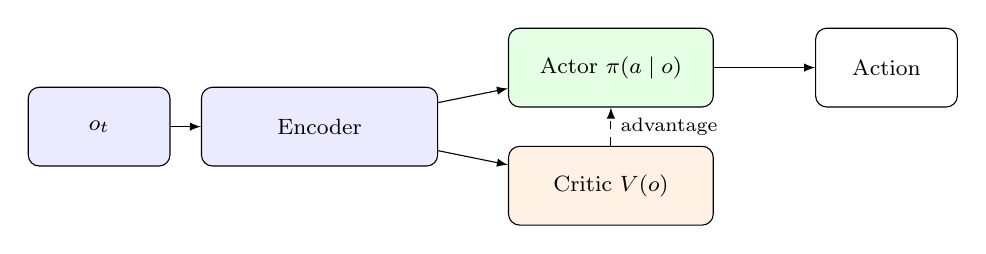
\begin{tikzpicture}[>=latex,font=\footnotesize]
\node[draw,rounded corners,fill=blue!8,minimum width=18mm,minimum height=10mm] (in) at (0,0) {$o_t$};
\node[draw,rounded corners,fill=blue!8,minimum width=30mm,minimum height=10mm] (enc) at (2.8,0) {Encoder};
\node[draw,rounded corners,fill=green!10,minimum width=26mm,minimum height=10mm] (a) at (6.5,.75) {Actor $\pi(a\mid o)$};
\node[draw,rounded corners,fill=orange!10,minimum width=26mm,minimum height=10mm] (c) at (6.5,-.75) {Critic $V(o)$};
\node[draw,rounded corners,minimum width=18mm,minimum height=10mm] (act) at (10,.75) {Action};
\draw[->] (in) -- (enc); \draw[->] (enc) -- (a); \draw[->] (enc) -- (c); \draw[->] (a) -- (act);
\draw[->,dashed] (c.north) -- node[right,font=\scriptsize]{advantage} (a.south);
\end{tikzpicture}}
\caption{Actor--critic data flow. The policy selects actions, while the critic supplies a lower-variance learning signal; actor and critic can share or separate encoders.}
\end{figure}
\textbf{PPO} constrains unusually large probability-ratio updates with a clipped surrogate objective:
\[
\underbrace{L_{\mathrm{PPO}}}_{\text{maximise}}
=\mathbb E\!\left[\min\!\left(
\underbrace{\rho_t A_t}_{\text{policy update}},
\underbrace{\operatorname{clip}(\rho_t,1-\epsilon,1+\epsilon)A_t}_{\text{cap improvement incentive}}\right)\right],\quad
\rho_t=\frac{\pi_{\theta}(a_t\mid o_t)}{\pi_{\mathrm{old}}(a_t\mid o_t)}.
\]
Clipping limits the surrogate incentive outside a ratio range, but does \emph{not} impose a strict trust region on the actual updated policy.
PPO implementations often combine policy loss, value regression and an entropy bonus; their coefficients, rollout length and number of optimisation epochs are experimental variables.
\textbf{SAC} instead maximises expected reward plus entropy while learning off-policy continuous-action critics, often trading more implementation complexity for greater experience reuse.

\subsection{Major Design Choices}\label{sec:rl-choices}
\begin{center}\begingroup\footnotesize\setlength{\tabcolsep}{3pt}
\begin{tabular}{|p{.24\linewidth}|p{.34\linewidth}|p{.33\linewidth}|}\hline
\textbf{Choice} & \textbf{When attractive} & \textbf{Main cost / failure}\\ \hline
Value-based / policy-based & Few discrete actions / continuous or structured actions & Maximising $Q$ becomes hard / high-variance gradients\\ \hline
Actor-only / actor--critic & Simpler estimator / lower variance from critic & Noisy returns / critic errors, more compute\\ \hline
On-policy / off-policy & Fresh rollout reflects current policy / replay scarce experience & Many interactions / distribution shift and correction\\ \hline
Model-free / model-based & Unknown dynamics / costly real-world interaction & Sample hungry / planning and model errors\\ \hline
Online / offline & Can explore live / only fixed logged dataset available & Exploration cost / out-of-distribution actions\\ \hline
Deterministic / stochastic & Low action sampling cost / exploration and multimodality & Narrow behaviours / entropy and sampling overhead\\ \hline
\end{tabular}\endgroup\end{center}
On-policy and off-policy concern \emph{which policy generated training experience}; online and offline concern \emph{whether new environment interaction is allowed}.
A model-based agent can use online or offline data; a critic may be fitted from either source, so these axes should not be treated as mutually exclusive algorithm categories.
An environment with partial observations also creates a representation choice: give the policy a recurrent memory, a fixed history window, or an explicit belief-state estimator.

\subsection{Modern RL Extensions}\label{sec:rl-extensions}
\textbf{Model-based RL} fits or uses transitions/rewards, then plans with methods such as model-predictive control (MPC) or generates synthetic rollouts.
A learned \textbf{world model} compresses observations into a latent dynamical state, allowing prediction and sometimes planning in a smaller space; long rollouts amplify modelling error.
\textbf{Imitation learning} copies demonstrations and does not require an online reward; behavioural cloning is supervised action prediction, whereas inverse RL attempts to infer the reward implied by behaviour.
\textbf{Offline RL} learns value/policy updates from fixed trajectories but must handle actions under-represented in the dataset, often through conservative objectives or constraints toward observed behaviour.
\textbf{Hierarchical RL} chooses temporal abstractions (skills/options) so decisions can operate at different timescales, trading extra structure for easier long-horizon control.
\textbf{Constrained RL} adds costs or safety budgets rather than hoping a single scalar reward penalty encodes every hard restriction.
\textbf{Multi-agent RL} introduces non-stationarity because other agents learn simultaneously; centralised training with decentralised execution is one response.

\subsection{Policy Research}\label{sec:rl-policy-research}
A policy is not synonymous with a simple action classifier: it may predict a deterministic control vector, parameters of a Gaussian, a token sequence, or an entire action trajectory generated iteratively.
The research question is both \emph{how to improve a policy} and \emph{what class of behaviours its parameterisation can represent}.

\begin{center}\begingroup\footnotesize\setlength{\tabcolsep}{3pt}
\begin{tabular}{|p{.22\linewidth}|p{.36\linewidth}|p{.33\linewidth}|}\hline
\textbf{Policy family} & \textbf{Structural assumption / inductive bias} & \textbf{Useful when / main cost}\\ \hline
Categorical / Gaussian & Actions arise from a simple conditional distribution & Cheap sampling; limited multimodality\\ \hline
Autoregressive & Complex action is assembled sequentially & Language/tool use; latency, stepwise errors\\ \hline
Recurrent / Transformer & History resolves ambiguity or sets long-range context & Partial observations; memory and context cost\\ \hline
Diffusion / flow policy & Sample complex, possibly multi-modal trajectories & Manipulation/action chunks; iterative sampling cost\\ \hline
Vision--language--action & Shared representation links images, instructions and robot actions & Cross-task transfer; data and deployment mismatch\\ \hline
Residual / parameter-efficient policy & Modify a pretrained controller instead of replacing it & Cheap adaptation; constrained new behaviour\\ \hline
\end{tabular}\endgroup\end{center}
\paragraph{Research evolution.}
REINFORCE estimates a direct policy update from trajectory return; actor--critic adds a learned baseline; TRPO/PPO limit destabilising jumps; DDPG/TD3/SAC bring off-policy replay into continuous control.
A newer, \emph{separate} branch begins with offline demonstrations, pretrained vision/language representations and generative policies, then optionally applies RL for reward-driven improvement.
Diffusion or flow matching is a \emph{policy representation/training mechanism}, not automatically RL: imitation-trained action generation can be followed by online reward optimisation.
This connects directly to the generative models in Chapter~16 and adaptation in Section~11.7.

\paragraph{Active research directions (2025--2026).}
\textbf{Expressive policies} model multi-modal action sequences, but iterative sampling competes with real-time control budgets; streaming or few-step policies reduce latency.
\textbf{Pretraining plus RL} begins with demonstrations or generalist policies rather than random behaviour, then asks how to improve success without losing previously learned skills.
\textbf{Scalable policy optimisation} studies asynchronous rollout systems, stale-policy correction, KL control and sample reuse, especially for large language models.
\textbf{Generalisation} targets changing tasks, scene geometry, robot embodiments and longer horizons, rather than repeatedly solving one fixed benchmark.
\textbf{LLM policies} require sequence-level rewards, long tool trajectories, verifiers and credit assignment for intermediate actions.
These are research directions, not a claim that one policy family has replaced all others.

\textbf{Current research anchors.} \emph{Streaming Flow Policy} (Jiang et al., CoRL 2025) changes how action trajectories are generated to allow earlier control execution; \emph{Flow-GRPO} (Liu et al., NeurIPS 2025) shows online policy-gradient improvement of a flow-matching generative model.
These results illustrate two different modifications: reduce \emph{inference-time action latency} versus change the \emph{training objective}.
The result in one generative domain does not establish superiority for robot control or language without task-specific evidence.
\paragraph{Action chunks and real-time control.}
A one-step policy repeatedly observes and chooses one action, giving high feedback frequency but requiring frequent model calls.
An action-chunk policy outputs $(a_t,\ldots,a_{t+K-1})$ per call, amortising expensive inference but risking stale control when the world changes within the chunk.
A receding-horizon controller executes only the first part of a predicted chunk and replans from the latest observation; that reduces open-loop drift but increases model calls.
This creates a measurable research axis: chunk length $K$, control frequency, prediction horizon and replanning cadence.

\textbf{Degree of Experiment.} Vary the action distribution (Gaussian / diffusion / flow), action chunk length, observation history, backbone, pretrained layers updated, KL/entropy strength, rollout freshness and environment randomisation.
Then measure success, interaction steps, compute cost, inference latency, diversity, and robustness separately; a higher reward from a richer policy may not justify a slower control cycle.
\begin{calloutintuition}
Policy representation determines which behaviours are expressible; policy optimisation determines which of them become likely.
\end{calloutintuition}

\subsection{RL for LLMs}\label{sec:rl-llms}
For an LLM, the \textbf{policy} is the conditional token distribution $\pi_{\theta}(y\mid x)$; $x$ is the prompt and $y$ a generated response, or a sequence of tool calls and observations.
The environment may return a preference score, a verifier result, or feedback from external tools; a whole-response reward makes assigning responsibility to individual tokens difficult.
Section~25.1.4 covers the classical RLHF workflow; Section~4.4 covers the pairwise ranking signal used to train reward models.

\begin{figure}[!htbp]\centering
\resizebox{.98\linewidth}{!}{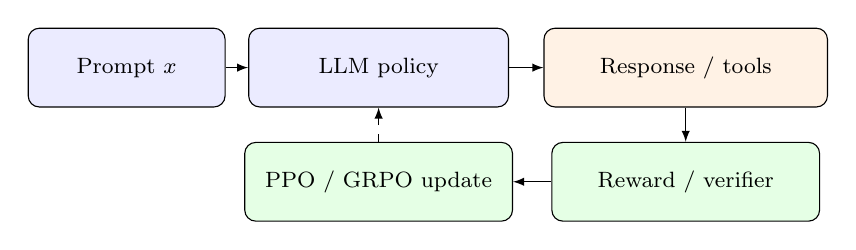
\begin{tikzpicture}[>=latex,font=\footnotesize]
\node[draw,rounded corners,fill=blue!8,minimum width=25mm,minimum height=10mm] (p) at (0,0) {Prompt $x$};
\node[draw,rounded corners,fill=blue!8,minimum width=33mm,minimum height=10mm] (m) at (3.2,0) {LLM policy};
\node[draw,rounded corners,fill=orange!10,minimum width=36mm,minimum height=10mm] (r) at (7.1,0) {Response / tools};
\node[draw,rounded corners,fill=green!10,minimum width=34mm,minimum height=10mm] (v) at (7.1,-1.45) {Reward / verifier};
\node[draw,rounded corners,fill=green!10,minimum width=34mm,minimum height=10mm] (u) at (3.2,-1.45) {PPO / GRPO update};
\draw[->] (p) -- (m); \draw[->] (m) -- (r); \draw[->] (r) -- (v); \draw[->] (v) -- (u);
\draw[->,dashed] (u) -- (m);
\end{tikzpicture}}
\caption{Online LLM RL gathers generations, evaluates them and updates the policy; DPO instead trains directly on existing preference pairs.}
\end{figure}
\begin{center}\begingroup\footnotesize\setlength{\tabcolsep}{3pt}
\begin{tabular}{|p{.18\linewidth}|p{.39\linewidth}|p{.34\linewidth}|}\hline
\textbf{Method} & \textbf{Training signal / mechanism} & \textbf{Key distinction}\\ \hline
SFT & Demonstration response and token cross-entropy & Imitates targets, no reward-driven exploration\\ \hline
RLHF + PPO & Learn preference reward, sample responses, clipped policy improvement, often KL to reference & Online policy optimisation; learned reward can be exploited\\ \hline
DPO & Pairwise chosen/rejected responses with preference classification loss & No explicit online RL rollout or separate reward-model training in standard DPO\\ \hline
GRPO / RLVR & Group responses to same problem; relative rewards/advantages; often verifiable correctness & Avoids separate value critic in common formulation; group sampling and reward design matter\\ \hline
\end{tabular}\endgroup\end{center}
\textbf{DPO is not an RL algorithm} in its usual offline preference-training form, although it is derived from a KL-regularised RLHF objective.
\textbf{GRPO} estimates within-group relative advantages instead of fitting a separate value critic, lowering critic memory but relying on informative group reward differences; without variation inside a group, the training signal may weaken.
For $N_{\mathrm{samples\ per\ prompt}}$ generated answers to the same prompt, a simple group-relative advantage is
\[
\underbrace{\widehat A_i}_{\text{relative quality of answer }i}
=\frac{\overbrace{r_i-\operatorname{mean}(r_1,\dots,r_N)}^{\text{compare against other responses}}}{\operatorname{std}(r_1,\dots,r_N)+\epsilon},\qquad N=N_{\mathrm{samples\ per\ prompt}}.
\]
The exact normalisation and objective vary by implementation; the mechanism is to compare samples from the same task instead of fitting a separate critic baseline.
\textbf{RL with verifiable rewards} (RLVR) substitutes checkable outcomes such as test results or exact answers for a subjective reward model where suitable; reward validity, hidden-test generalisation and specification gaming remain problems.
A KL penalty against a reference policy reduces unconstrained drift; its coefficient trades task-reward improvement against deviation from previously learned behaviour.

\subsection{Research Practice, Failure Modes and Evaluation}\label{sec:rl-research-practice}
An RL experiment must version \emph{environment code, policy code, reward function, simulator settings, reset distribution, seed and evaluation protocol}; a model checkpoint alone is not the experiment.
Report environment interactions and wall-clock/GPU costs separately: replay or modelling may improve sample efficiency while increasing computational expense.
Compare both final and learning-curve performance across multiple seeds, using matched environment steps or matched compute budgets according to the research question.
Do not use training reward alone as evidence of behaviour quality: test independent success criteria, violations and generalisation to altered tasks.
\textbf{Experiment design.} Fix the observation/action spaces and evaluation seeds, compare a tabular or heuristic baseline where possible, change one method component, and repeat across seeds.
Ablate reward shaping, entropy regularisation, target-network update interval, replay size, GAE parameter and action chunk length only where they are actually used; otherwise a large hyperparameter search may obscure the causal change.
In stochastic tasks report uncertainty on success/return and distinguish \emph{within-environment variation} from \emph{training-seed variation}.
\textbf{Evaluation leakage} occurs when the agent learns a fixed reset pattern, sees privileged simulator state unavailable at deployment, or encounters its held-out tasks during curriculum generation.
For simulator-to-real transfer, test parameter shifts and sensor corruption before deployment; offline logs alone do not establish closed-loop performance.

\begin{center}\begingroup\footnotesize\setlength{\tabcolsep}{3pt}
\begin{tabular}{|p{.23\linewidth}|p{.38\linewidth}|p{.30\linewidth}|}\hline
\textbf{Observed failure} & \textbf{Likely mechanism} & \textbf{First diagnostic}\\ \hline
Reward rises; task success does not & Reward proxy exploits / specification mismatch & Inspect trajectories and independent success metric\\ \hline
Values explode or oscillate & Moving bootstrapped targets; large updates; scale & TD error, target lag, gradient / Q norms\\ \hline
Policy entropy collapses & Early exploit, weak exploration or excessive policy shift & Entropy, action histogram, reward coverage\\ \hline
Training good; transfer poor & Narrow reset distribution, simulator bias or leakage & Held-out seeds, perturb dynamics, mask privileged state\\ \hline
Throughput low & Environment stepping, tool latency, serial sampling & Profile step/inference/queue/update time\\ \hline
Offline policy fails online & Actions leave behaviour-data support & Action support, OOD critic estimates\\ \hline
\end{tabular}\endgroup\end{center}
\textbf{Two worked designs.} \emph{Cart-pole control}: observe position/velocity/angle, choose a left/right force and reward sustained balance; change observation noise, control frequency or termination and compare DQN with PPO under fixed interactions.
\emph{LLM post-training}: produce multiple answers, score by preference or a verifier, and compare SFT, DPO and online PPO/GRPO on an untouched test suite; track correctness, KL drift, sampling compute, answer diversity and failure cases rather than reward alone.

\textbf{Researcher diagnostic.} When selecting an RL method, ask in order: \emph{What is controllable? What is observable? Who defines reward? Is interaction cheap? Are actions discrete, continuous or structured? Do we need exploration? What experience may be reused? What metric verifies success independently of reward?}
The general failure mode is optimising an imperfect task definition more effectively than the task itself.

% Compact source anchors for contemporary API / policy claims, without depending
% on the textbook's bibliography keys. Official documentation / original papers:
% Gymnasium: https://gymnasium.farama.org/api/env/
% PettingZoo: https://pettingzoo.farama.org/
% MuJoCo MJX: https://mujoco.readthedocs.io/en/stable/mjx.html
% Isaac Lab: https://developer.nvidia.com/isaac/lab
% BrowserGym: https://github.com/ServiceNow/BrowserGym
% PPO: Schulman et al. (2017), arXiv:1707.06347
% DPO: Rafailov et al. (2023), arXiv:2305.18290
% GRPO: Shao et al. (2024), arXiv:2402.03300
% Streaming Flow Policy: Jiang et al., CoRL 2025, PMLR 305.
% Flow-GRPO: Liu et al., NeurIPS 2025.